%%%%%%%%%%%%%%%%%%%%%%%%%%%%%%%%%%%%%%%%%%%%%%%%%%%%%%%%%%%%%%%%%%%%%%%%%%%%%%%%
%2345678901234567890123456789012345678901234567890123456789012345678901234567890
%        1         2         3         4         5         6         7         8

\documentclass[letterpaper, 10 pt, conference]{ieeeconf}  % Comment this line out
                                                          % if you need a4paper
%\documentclass[a4paper, 10pt, conference]{ieeeconf}      % Use this line for a4
                                                          % paper

\IEEEoverridecommandlockouts                              % This command is only
                                                          % needed if you want to
                                                          % use the \thanks command
\overrideIEEEmargins
% See the \addtolength command later in the file to balance the column lengths
% on the last page of the document



% The following packages can be found on http:\\www.ctan.org
\usepackage{graphicx} % for pdf, bitmapped graphics files
%\usepackage{epsfig} % for postscript graphics files
%\usepackage{mathptmx} % assumes new font selection scheme installed
%\usepackage{times} % assumes new font selection scheme installed
\usepackage{amsmath} % assumes amsmath package installed
\usepackage{amssymb}  % assumes amsmath package installed

\title{\LARGE \bf
Planning and Control Under Uncertainty for the PR2
}

%\author{ \parbox{3 in}{\centering Huibert Kwakernaak*
%         \thanks{*Use the $\backslash$thanks command to put information here}\\
%         Faculty of Electrical Engineering, Mathematics and Computer Science\\
%         University of Twente\\
%         7500 AE Enschede, The Netherlands\\
%         {\tt\small h.kwakernaak@autsubmit.com}}
%         \hspace*{ 0.5 in}
%         \parbox{3 in}{ \centering Pradeep Misra**
%         \thanks{**The footnote marks may be inserted manually}\\
%        Department of Electrical Engineering \\
%         Wright State University\\
%         Dayton, OH 45435, USA\\
%         {\tt\small pmisra@cs.wright.edu}}
%}

\author{Jennifer Barry, Mario Bollini, Anne Holladay, Leslie Pack
  Kaelbling, Tom\'{a}s Lozano-P\'{e}rez%
\thanks{All authors are with CSAIL,
  MIT.}% 
\thanks{{\tt \{jbarry,mbollini,holladay,lpk,tlp\}@csail.mit.edu}}%
}


\begin{document}



\maketitle
\thispagestyle{empty}
\pagestyle{empty}


%%%%%%%%%%%%%%%%%%%%%%%%%%%%%%%%%%%%%%%%%%%%%%%%%%%%%%%%%%%%%%%%%%%%%%%%%%%%%%%%
\section{INTRODUCTION}

The
quality of robotic sensors and actuators has improved dramatically 
in the last decade to the point that robots are now physically able
to run for days without human intervention.  However, tasks that
span hours or days require planners and controllers capable of dealing
with long time-horizons and high uncertainty.
In this abstract, we present our progress towards the goal of planning
and 
executing complex tasks in uncertain
environments.
We begin by discussing our
hierarchical planning algorithm designed to work on tasks with
potentially very long horizons and complicated, uncertain geometric
sub-tasks.  We then focus on the geometric sub-tasks, 
showing that force control is useful for tasks where
uncertainty makes position control difficult or impossible.

\section{HIGH-LEVEL PLANNING WITH THE PR2}

In order for a robot to carry out complex tasks, it must be able to
reason about long time scales, abstract ideas, and uncertainty.   
We believe this requires an integration of symbolic and geometric
planning.  Symbolic task planners and
geometric motion planners have complementary strengths.  Task planners
can reason about large, partially specified state spaces and return
plans on these partial states covering a 
long time scale; conversely, geometric planners require a full
specification of the state but return a plan at the geometric level.
A task planner decides that a cup needs to be picked up; the geometric
planner must be employed to decide how.

The Hierarchical Planning in the Now (HPN) framework is an algorithm
for integrating task planning and geometric motion planning.  It is
aggressively hierarchical, committing early to geometric
plans and interleaving planning and execution.  By utilizing symbolic
planners at the upper levels of the hierarchy and geometric planners
at the lowest level, the planner operates in the space of continuous
geometry, requiring no a priori discretization of the state space, and
integrates reasoning about information gathering tasks.  By coupling
some
high-level reasoning about uncertainty with an aggressive re-planning
routine, the planner is able to perform well even in highly uncertain
situations.

At the symbolic level, a plan is a sequence of operations.  An
operation consists of a pre-condition and effect, represented
symbolically, and a primitive refinement for executing the operation.
For example, consider the operation of {\sc Place}ing an
object $O$ in region $R$.  We use four fluents: 
(1) {\tt Scanned} indicates that we have scanned the environment and
  located objects in it,
(2) {\tt ClearX}($M$, $L$) indicates that motion $M$ is
  collision-free except for objects in the list $L$,
(3) {\tt In}($O$, $R$) indicates that object $O$ is in region $R$,
and (4) {\tt Holding}($O$) indicates that the robot is holding object
  $O$.
Before placing object $O$ in region $R$, we must have scanned the
environment, have picked up
object $O$, and have some free path for placing object $O$.
Therefore, the pre-condition for {\sc Place} is ({\tt
  Scanned} $\wedge$ {\tt ClearX}(PlaceMotion, $\{O\}$)
$\wedge$ {\tt Holding}($O$)) and the effect is {\tt In}($O$, $R$).
The primitive refinement is planning and following the
geometric path to
actually place the object.

Note that by making {\tt Scanned} a pre-condition for {\sc Place}, we
have automatically integrated information gathering, assuring that any
plan that wishes to place an object will first locate it in the
environment.  For more
complicated
domains we could reason more explicitly about uncertainty,
requiring that we know the position of the object we want to
place to some accuracy and with some confidence.  This would lead the
algorithm to continue gathering information until the accuracy and
confidence conditions were met.


To create a hierarchy, we choose an ordering of the pre-conditions
that reflects the serializability of the domain.
For example, for {\sc Place}, we could choose the ordering:
\begin{itemize}
\item[0)] {\tt Scanned}
\item[1)] {\tt Holding}($O$)
\item[2)] {\tt ClearX}(PlaceMotion, $\{O\}$)
\end{itemize}
This hierarchy indicates that we should first plan to have scanned the
environment, then to have scanned the environment
{\em and} be holding object $O$, and lastly, to have scanned the
environment, be holding object $O$, and have a clear path to place
object $O$.  A diagram of a possible plan using this hierarchy is
shown in
Figure~\ref{fig:hierarchy}. Before considering a sub-task, all
previous sub-tasks in the plan are fully planned for and executed.
However, if a pre-condition for a sub-task were to become false, we
would re-plan for that pre-condition, allowing us to compensate both
for uncertainty and for 
incorrect hierarchies.  Because we re-plan whenever a pre-condition
becomes 
false and the last goal of the hierarchy is the flat goal originally
specified,
provided all actions in the domain are reversible, we will eventually
succeed at the task.


\begin{figure}
\centering
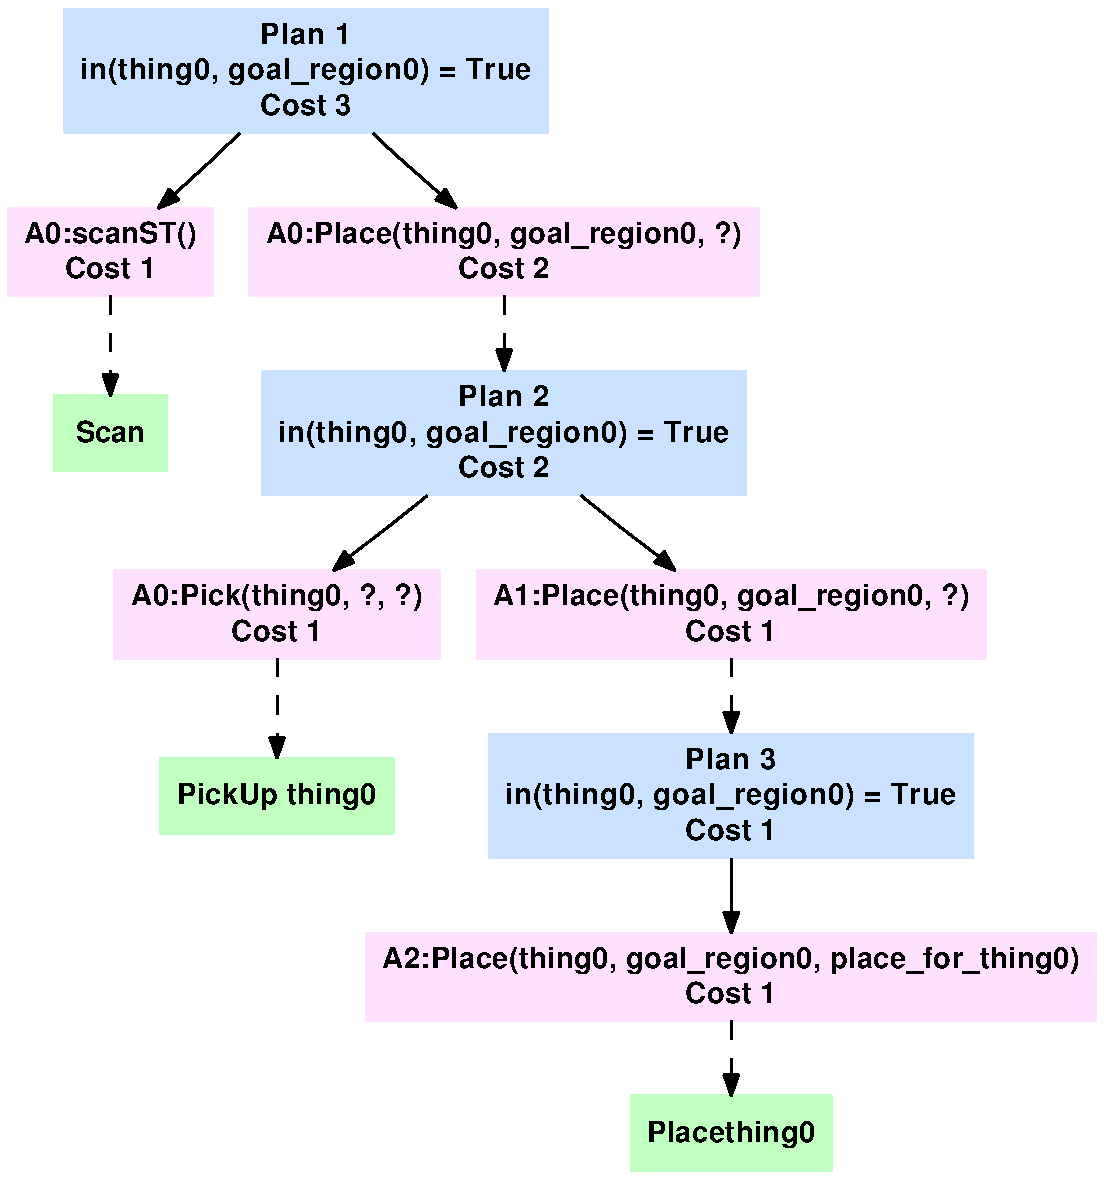
\includegraphics[height=3in]{images/pr2.pdf}
\caption{A plan for executing a simple place task of one object.
  Goals are shown in blue, operators in purple, and primitive actions
  in green.  Plans are executed left to right.  The plan at the
  first level of 
hierarchy first requires that the environment be {\tt Scanned}.
Therefore,
before considering anything else, we first {\sc Scan} the
environment.  Once that is done, we consider the next level of the
{\sc Place} sub-task, which requires that we be {\tt Holding} the
object and
fully plan and execute picking up the object.  Finally, we plan
for placing
the object.  Since we only have one object in this
environment, the place motion is already clear and that branch
requires no plan.}
\label{fig:hierarchy}
\end{figure}


By using the hierarchy to serialize sub-tasks, we can interleave
planning and execution, reducing the size of the search space.  For
example, when placing an object, the {\tt Holding} pre-condition is
ordered before the {\tt ClearX} pre-condition.  Therefore, the place path
is not planned until the robot is actually holding the
object.  Hence, we are planning in the
``now'': we already know exactly where and how the object will be held
at the moment before we begin the place.  Thus, we
know, for example, the grip the robot is employing; we do not need
to plan several different place paths for each possible grip.
This also keeps us from having to
discretize the possible grips when planning place paths.

We have implemented the HPN algorithm for a pick-and-place domain on
the
PR2 robot and have shown that it can plan and execute complicated
pick-and-place tasks.


\section{COMPLIANT CONTROL OF THE PR2}

In accomplishing long-horizon, uncertain tasks, the robot must
have 
the physical capability to carry out uncertain and complicated
geometric tasks.  In the last section we discussed how to sequence
these geometric tasks in a high-level plan.  Here, we focus on methods
for accomplishing each task in a robust fashion.

Many robots rely solely on position control to work with objects in
the world.  However, there are tasks where the force the robot exerts
is more important than its position.  Any task that requires a robot
to maintain
contact with a surface, for instance, is difficult or in some cases
impossible to accomplish using position control.  For
example, in wiping a table, the robot must be in contact with the
table at all times, but must press on the table using only a light
force.
This is a difficult task using position control as it requires precise
knowledge about the shape and placement of the table.  With force
control, however, we can
compensate for uncertainty in the height of the table by
just exerting a light downwards force until contact is felt with the
table.  By continuing to exert a light downwards force while wiping
the table, we are able to accomplish the task without ever explicitly
representing the height of the table.

Although the PR2 arms are compliant, there is no mechanism for
directly controlling force or impedance.  We have
written a controller that allows a user to request 
force/impedance trajectories.  Each point on the trajectory specifies
a wrench or stiffness around each Cartesian degree of freedom, as well
as a Cartesian point and orientation.  For a degree of freedom, if a
stiffness is specified, the controller will attempt to reach the
position given using that stiffness.  If a wrench is specified, the
position information is ignored.

The controller is an open-loop Jacobian-transpose force controller.
At each point on the trajectory, desired stiffness is converted to
a Cartesian wrench.  The Cartesian wrench vector is
then converted to a joint torque vector using the transpose of the
arm's instantaneous Jacobian matrix.
Because the controller is open-loop, we cannot make guarantees about
the magnitudes of the output wrench.  Joint stiction, joint
position limits, and motor torque limits may cause
the applied 
force/impedance to deviate from the desired values.  However,
we have found that although we cannot use precise forces, the ability
to use light force and to guarantee that some force will be
exerted in a Cartesian direction is useful.  We have demonstrated that
the controller can be used for drawing with a pencil, erasing,
sweeping, stirring, cutting a cake, wiping a table, and turning a page
of a notebook.

We have also found that force control is useful in tasks where a
purely position control solution is possible but difficult to
calculate.  For example, in opening a
cupboard or oven, we have shown 
that using a combination of force and position control allows us to
bypass planning the constrained path.  Assume we have a door that
opens around the $-y$ axis.  The trajectory to open the door follows a
path that is a piece of a circle on the $xz$-plane.  Rather than try
to calculate this circle, we only specify an ending point in $x$ and
just exert a force 
in the $-z$ direction.  We use a small stiffnesses in the remaining
four degrees
of freedom to allow the arm some freedom of movement around the
wrist.  This results in a successful opening that is
robust to small uncertainties.  Since we do not need to calculate a
full constrained trajectory, there is essentially no planning
time required.

The controller has been wrapped in a ROS action server for ease and
safety of use, and the code has been released.  Documentation is
available on the ROS wiki.

\section{Conclusions and Future Work}

Our goal is to make robots capable of carrying out complex tasks in
highly uncertain environments.  To this aim, we are developing both a
high-level algorithm 
that plans symbolically in long-horizon, uncertain domains and a
force/impedance controller that allows users to do force control on
the PR2 arms.  

We are working towards combining these capabilities, using the
high-level planner to find sub-goals for the force/impedance
controller.  We are also considering methods for learning models of
the PR2 arm joint stiction to make the force/impedance controller more
accurate and attempting to increase the efficiency of the HPN
searches using cost models of the search tree.


\end{document}
